\section{Introduction}

Robots are frequently used in remote and unpredictable environments.
%
% One trouble of using robots in these environments is that they must be capable of navigating highly varied terrain.
%
For example, in \emph{search and rescue} a robot is designed to aid first responders search for victims by traveling over highly varied terrain~\citep{Graf.2017.2ISSCIS.RescuePathOptimization}.
%
One solution to this problem is to use an unmanned aerial vehicle (UAV). However, UAVs can typically only operate for short periods of time (roughly 30 minutes to one hour).

\begin{figure}[!ht]
    \centering

    \subfloat[Physical Simulation]{%
        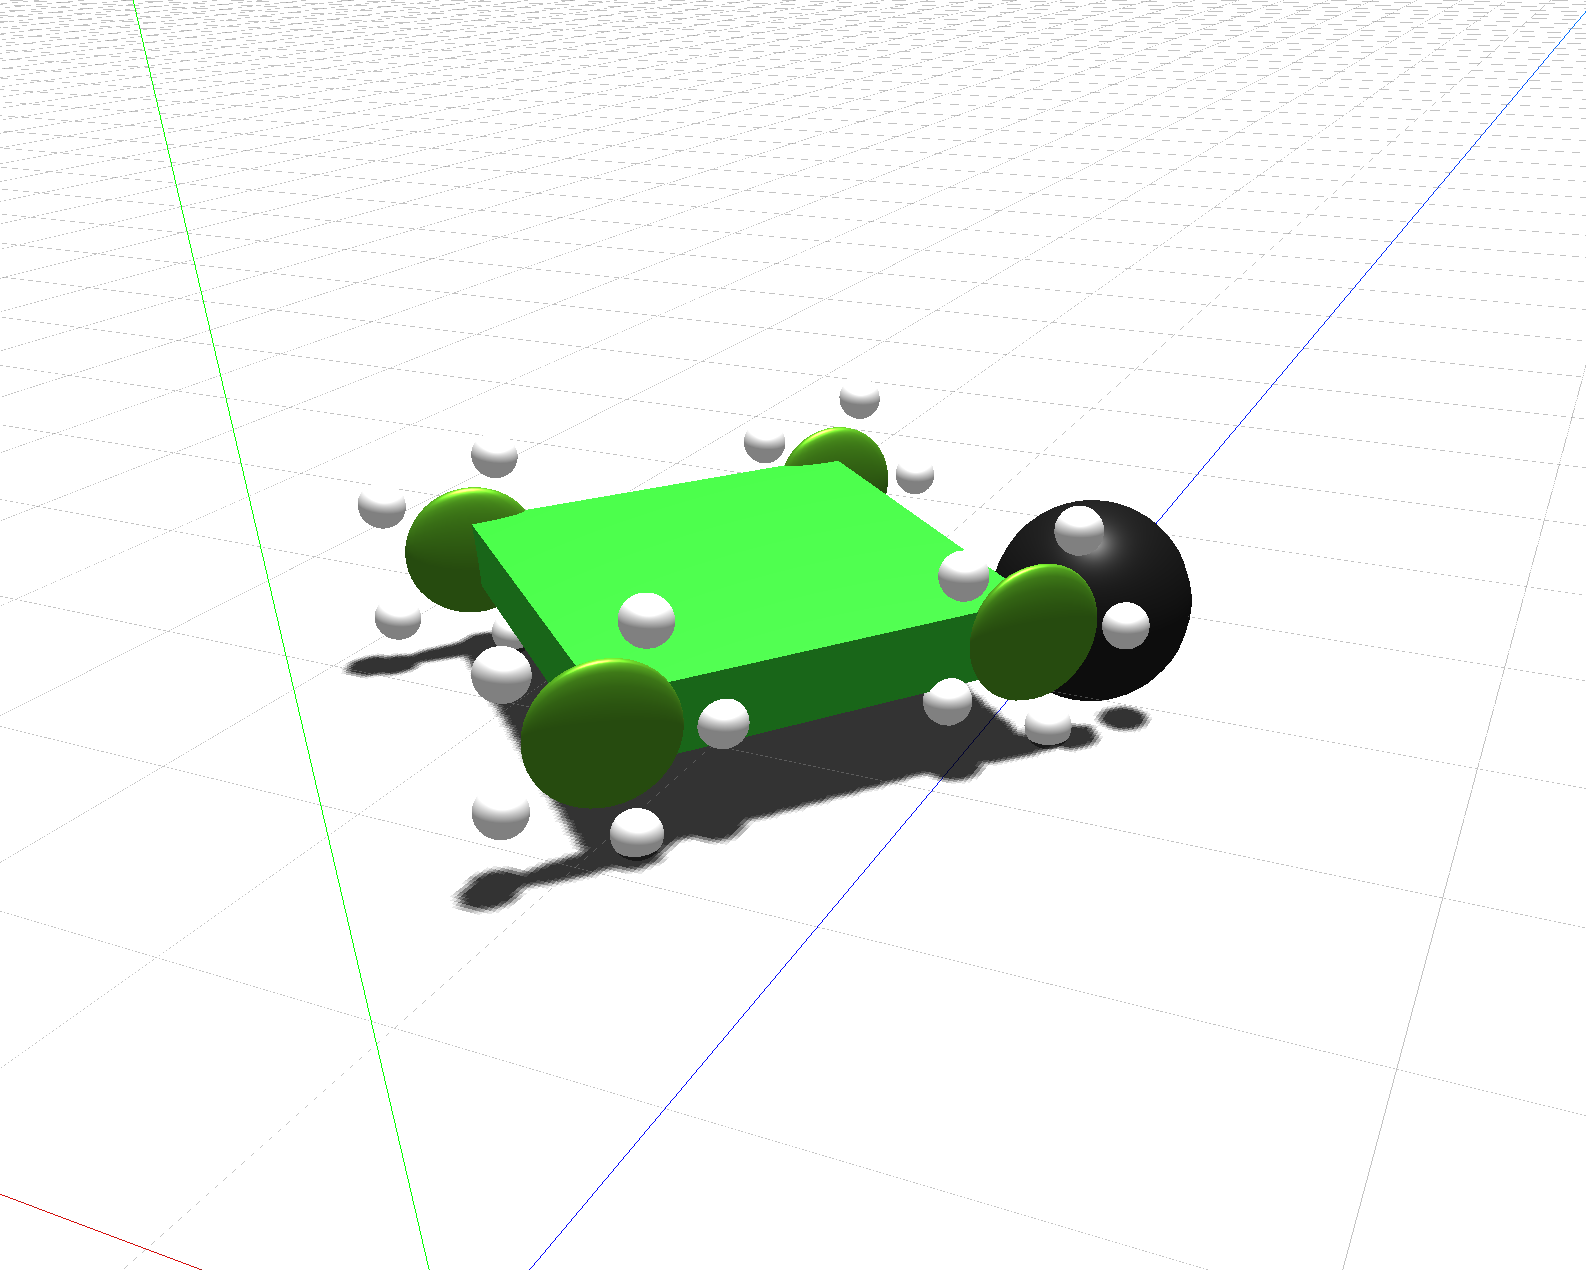
\includegraphics[width=0.4\columnwidth,valign=c]{figures/physical-simulation.png}%
        \vphantom{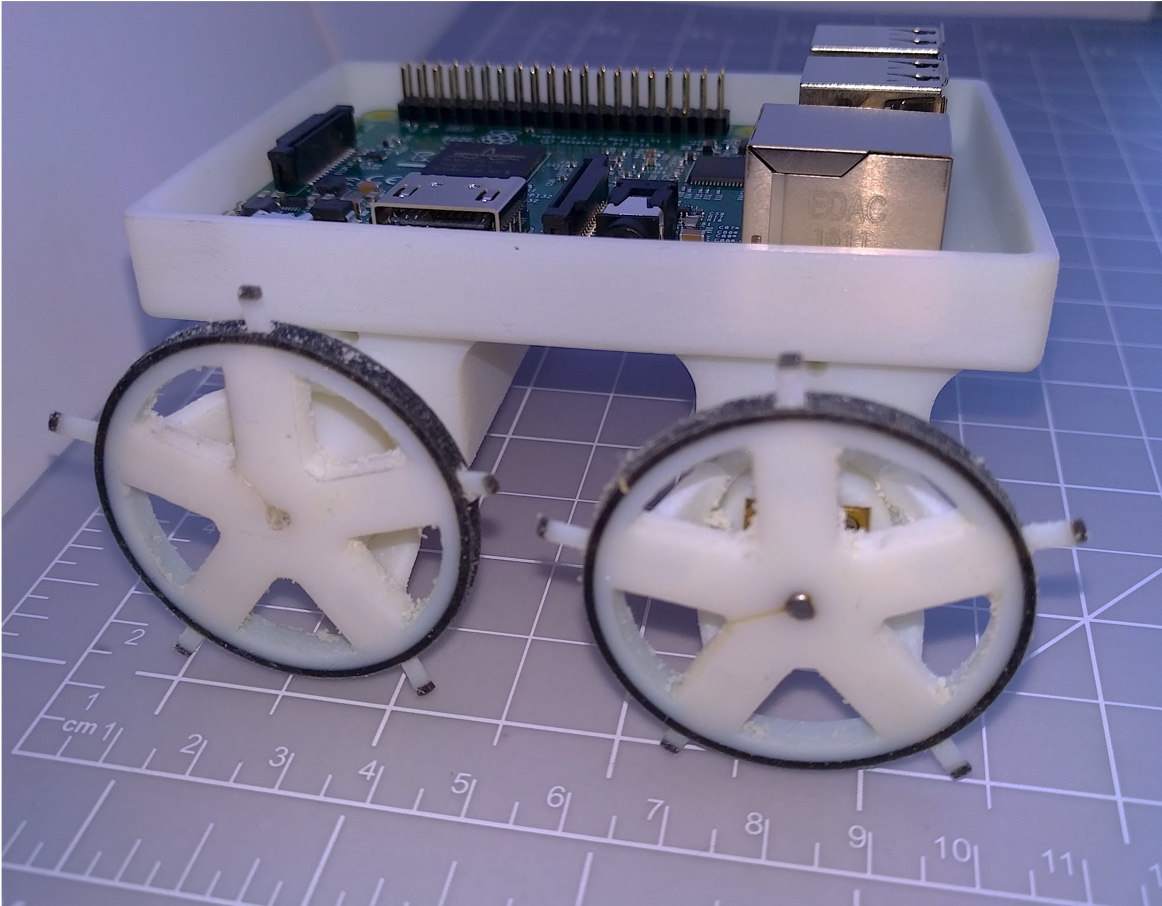
\includegraphics[width=0.4\columnwidth,valign=c]{figures/perspective-image.jpg}}%
    }\quad
    \subfloat[Prototype]{%
        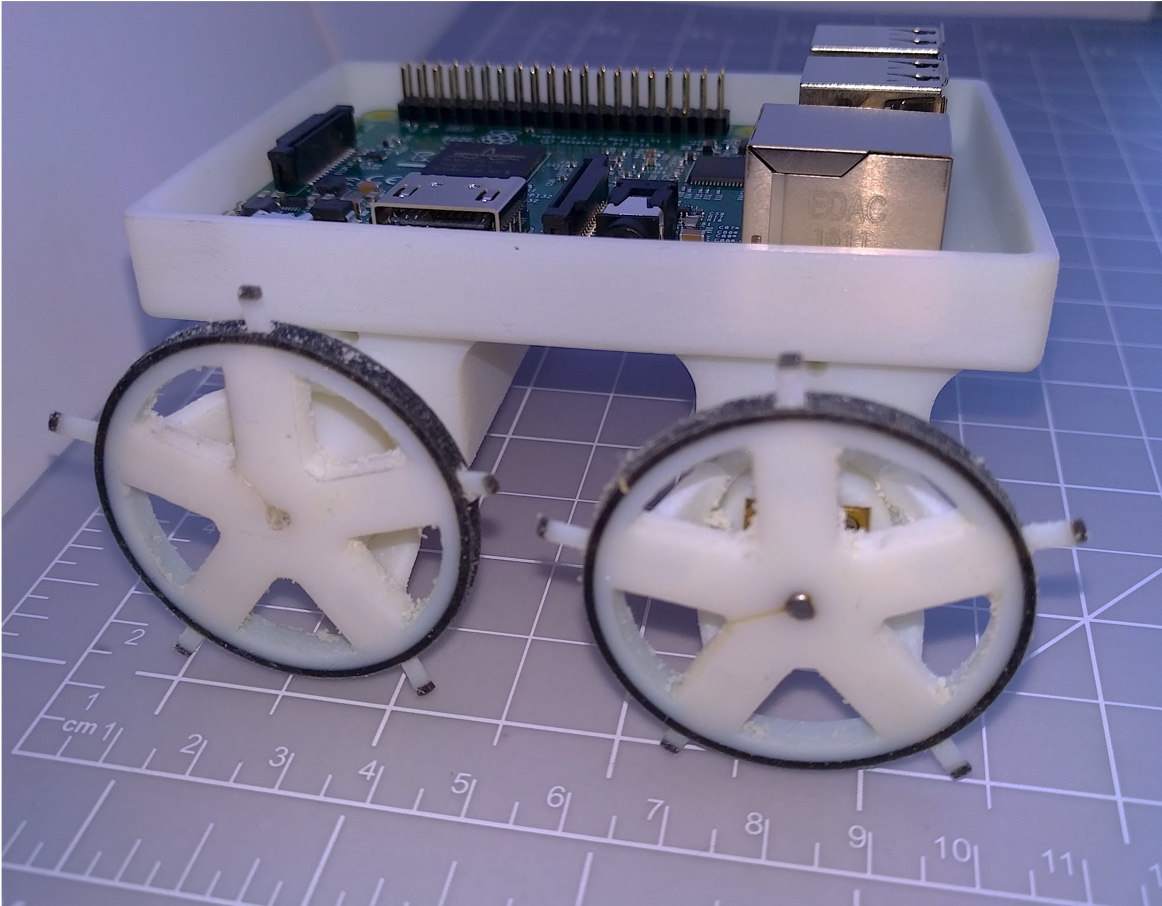
\includegraphics[width=0.4\columnwidth,valign=c]{figures/perspective-image.jpg}%
    }

    %\vspace{-0.05in}

    \caption{A mobile robot with transformable wheels (see the following an interactive visualization: \url{https://review.github.io/}).}
    \label{fig:robot}

    %\vspace{-0.15in}

\end{figure}

\begin{figure*}[ht]
    \centering
    \subfloat[]{%
        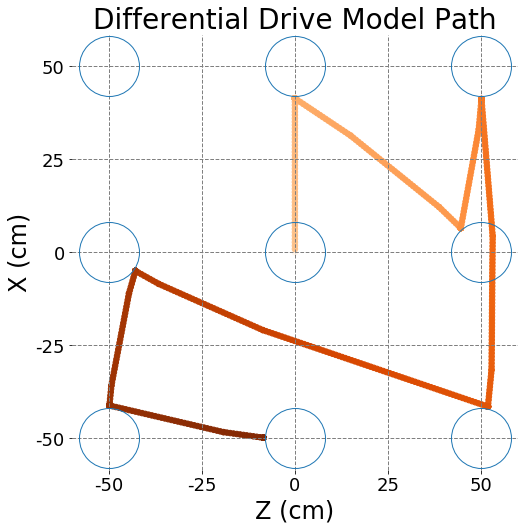
\includegraphics[height=1.6in]{figures/ddm-path.png}%
    }\hfil
    \subfloat[]{%
        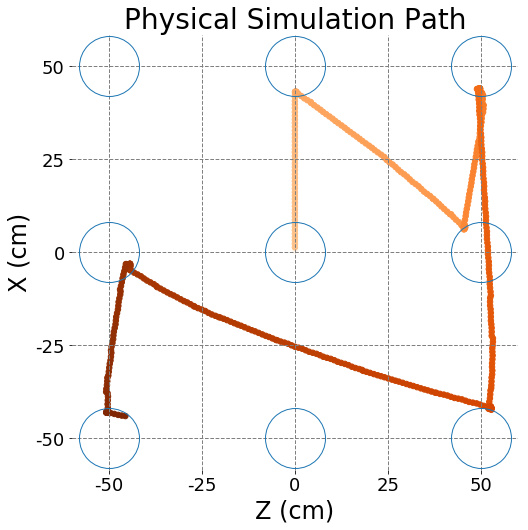
\includegraphics[height=1.6in]{figures/phy-path.png}%
    }\hfil
    \subfloat[]{%
        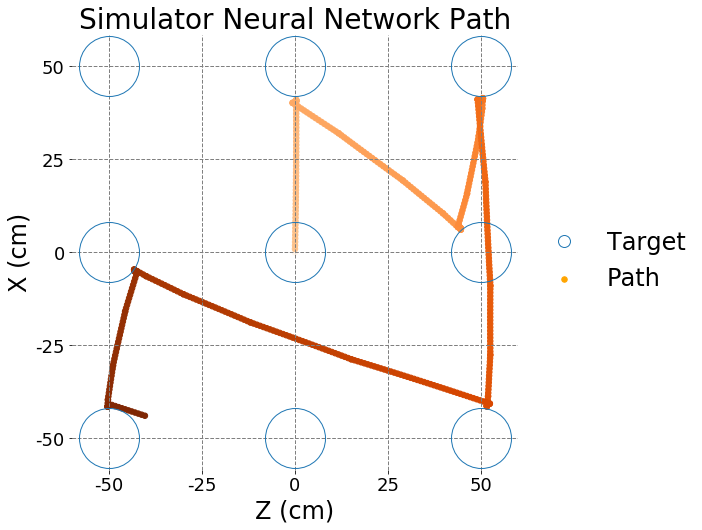
\includegraphics[height=1.6in]{figures/snn-path.png}%
    }
    %\vspace{-0.05in}
    \caption{Example paths taken by the robot (a) as predicted by the differential drive model, (b) during a physical simulation, and (c) as predicted by a trained SNN. Blue circles indicated way-points that the robot is trying to reach in a predefined sequence. The robot moves on to its next way-point once it gets within 10\si{cm} of the current way-point. Paths are indicated in orange, and lighter shades indicate earlier an earlier time (the robot starts at the origin).}
    \label{fig:paths}
    %\vspace{-0.15in}
\end{figure*}

More recently, lightweight mobile robots with transformable wheels have been developed for search and rescue.
%
As shown in Figure~\ref{fig:robot}, a transformable wheel robot is capable of extending struts radially outward from the center of each wheel. These struts help the robot climb over obstacles that are roughly the same size as the robot~\citep{Clark.2018.C.EvolvingControllersTransformable}.
%
These devices have the benefits of normal wheels (e.g., increased stability and less vibration) and legged-wheels (e.g., increased mobility), and they have a longer operating duration compared to UAVs.


A drawback of using a transformable wheel mobile robot (or a legged-wheel robot) is that they are difficult to model.
%
Without an accurate model of the robot, it is difficult to determine when wheels should be transformed from normal wheels into a legged-wheels.
%
Specifically, a model can be used to calculate the \emph{expected} velocity of the robot, and this quantity can be compared to the \emph{measured} velocity (using sensor readings). If these two quantities differ by some threshold amount, then the robot should infer that it is stuck or slipping and it should extend its wheel struts.
%
Without an accurate model of the robot kinematics, this process cannot work.


\noindent
\textbf{Related work.}
%
In prior work, we used a differential drive model to calculate \emph{expected} velocity~\citep{Clark.2018.C.EvolvingControllersTransformable}. This process was error prone.
%
The model did not account for strut extension, wheel slippage (i.e., differing friction properties of different terrains), uneven ground, or that the wheels might rotate at a different rate than commanded.
%
In this study, we develop a simulator neural network (SNN) similar to that described by \citet{Pretorius.2014.2ICECC.ComparisonNeuralNetworks}, where they train a neural network so that control signals map to changes the the pose of the robot.
